\documentclass[12pt]{article}
 
\usepackage[margin=1in]{geometry} 
\usepackage{amsmath,amsthm,amssymb,bm}
\usepackage{graphicx}
\usepackage{subcaption}
\usepackage{placeins}
\setlength{\parskip}{1em} %Paragraph spacing
 
\begin{document}
  
\title{Visual Understanding 1 Coursework}
\author{Garoe Dorta-Perez\\
CM50248: Visual Understanding 1\\
Unit Leader: Peter Hall\\
Bath University}
 
\maketitle
 
\section{Introduction}

The main objectives of this unit are to acquire the fundamentals of Computer Vision.
In order to gather this skills, we will attempt to build a stereo reconstruction system.
Using a bottom-up approach the following steps will be taken:
\begin{enumerate}
\item Image convolution, transforming using kernel matrices.
\item Feature construction, detecting scale invariant interest points in images.
\item Matching, using the previous points to match two images.
\item Stereo reconstruction, rebuilding 3D points from 2D matched points in stereo images.
\end{enumerate}

\section{Literature review}


\section{Convolution}
\label{sec:convolution}

Transforming images has artistic and practical applications, for instance blurring certain parts in a person face to hide defects or detecting borders with differential operators.
For simplicity we will restrict ourselves to gray images, defined as two-dimensional $n \times m$ matrices where each element represents the intensity, and is in the range $\lbrace  0, 1 \rbrace$ where 0 is black and 1 is white.
A convolution kernel $k$, is defined as a $k_1 \times k_2$ matrix, such that $k_1 \leqslant n$ and $k_2 \leqslant m$.
When an image $I_0$ is convoluted with a kernel, a new image $I_1$ is generated, such that each element in the second image is calculated as follows WRITE IT AS EQUATION OR EXPLAIN IT OTHERWISE.
The advantage in this definition is that, it gives a common framework for every possible transformation; so we only need to change the kernel to fit our needs.
However, we need to specify what will happen to the borders of the matrix, leave them as they are, set them to zero, compute circularly, etc; and where does the convolution start with kernel with an even number of columns or rows.

An interesting property of convolutions is the \emph{convolution theorem}, which states that $g * h = F^{-1} ( F(g) \cdot F(h) ) $.
This property allows to transform the images into the Fourier domain, apply the convolution, transform back and obtain the same results with less computational cost.
Below we show some examples of our convolution code, as well as a table comparing the performance of our initial code, our code with the Fourier transform and Matlab's implementation.

\begin{figure}[htbp]
        \centering
        \begin{subfigure}[b]{0.32\textwidth}
                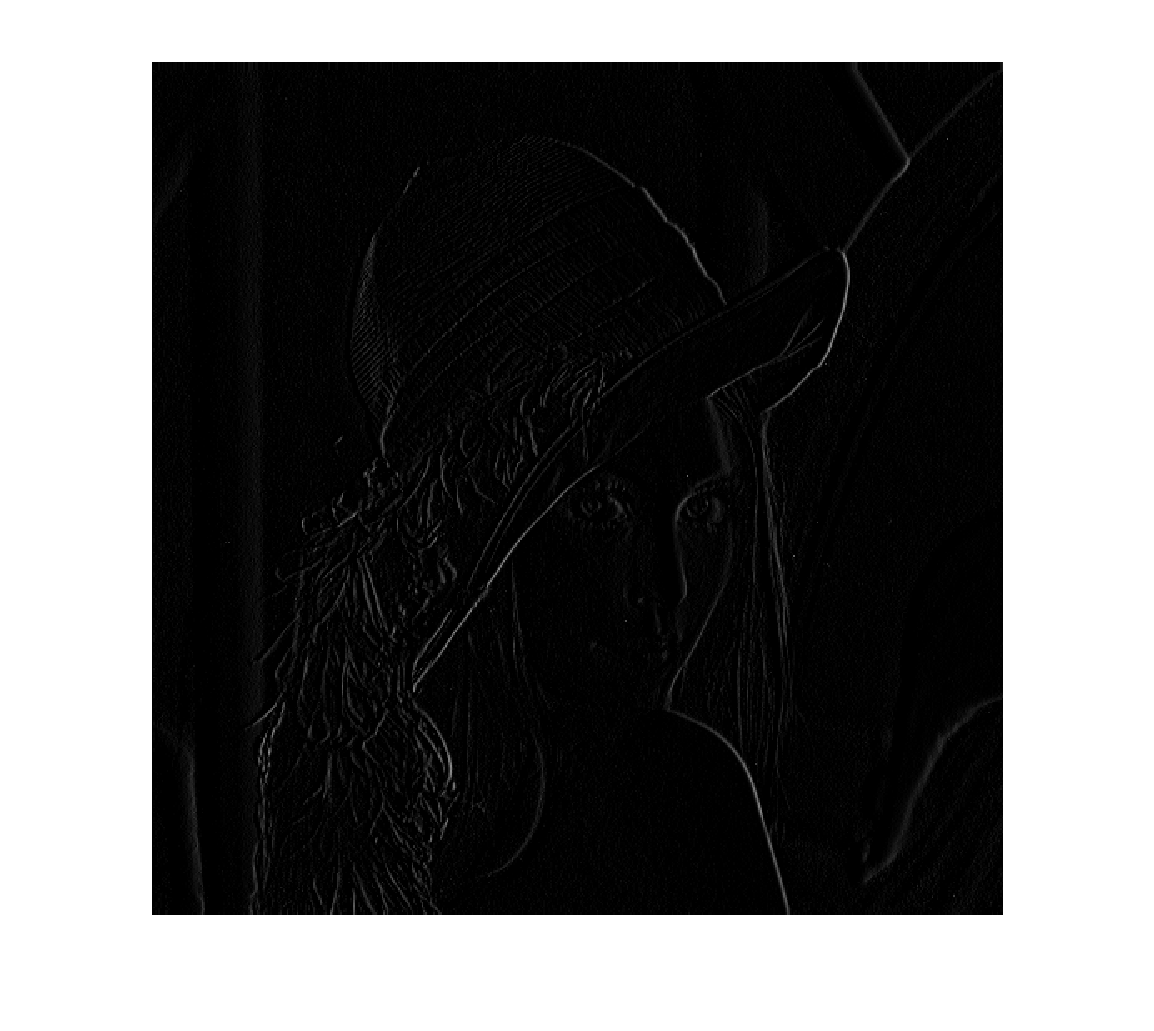
\includegraphics[width=\textwidth]{images/conv1}
                \caption{myconv.}
                \label{fig:myconv}
        \end{subfigure}
        \begin{subfigure}[b]{0.32\textwidth}
                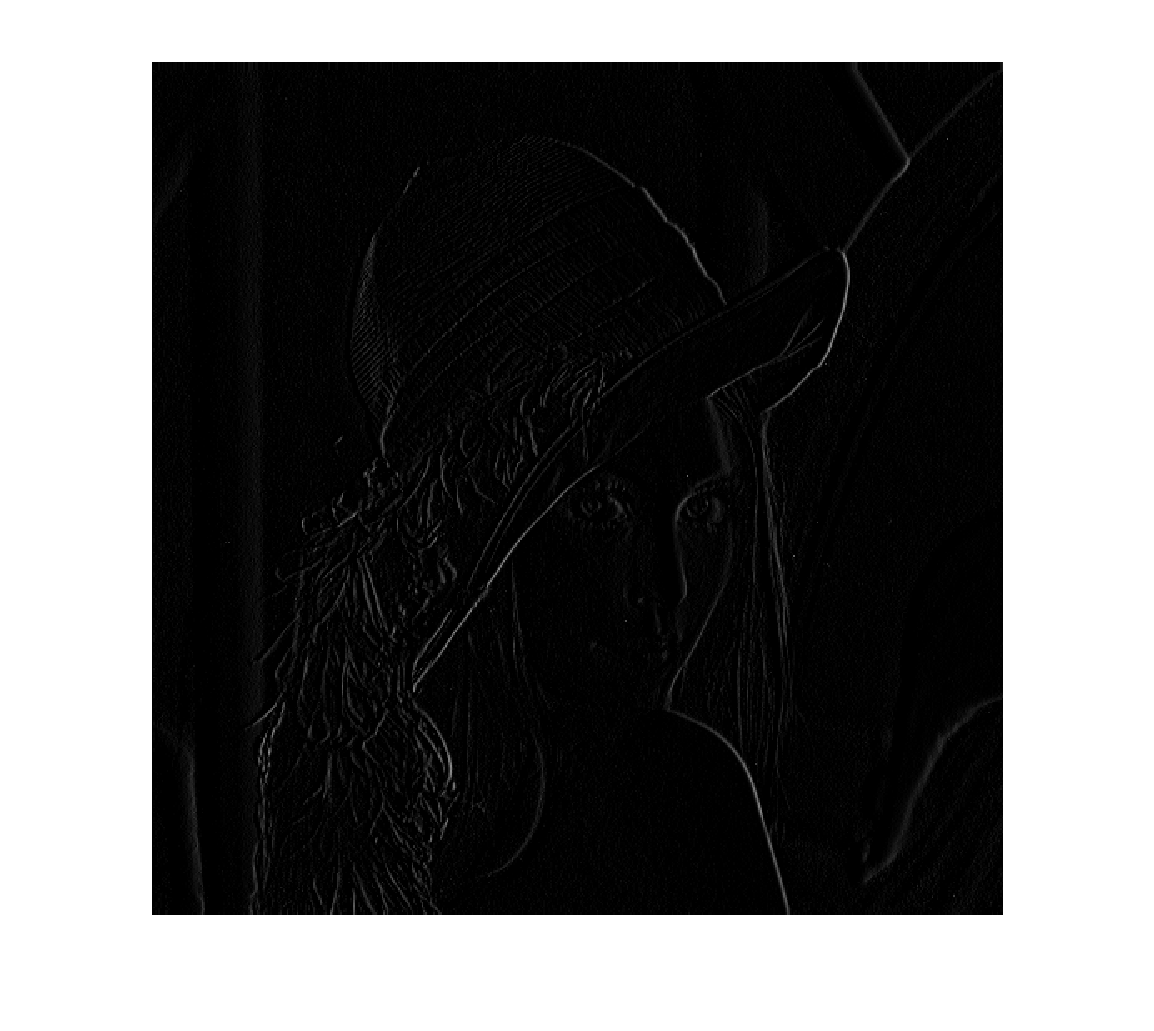
\includegraphics[width=\textwidth]{images/conv2}
                \caption{myconvFFT.}
                \label{fig:myconvFFT}
        \end{subfigure}
        \begin{subfigure}[b]{0.32\textwidth}
                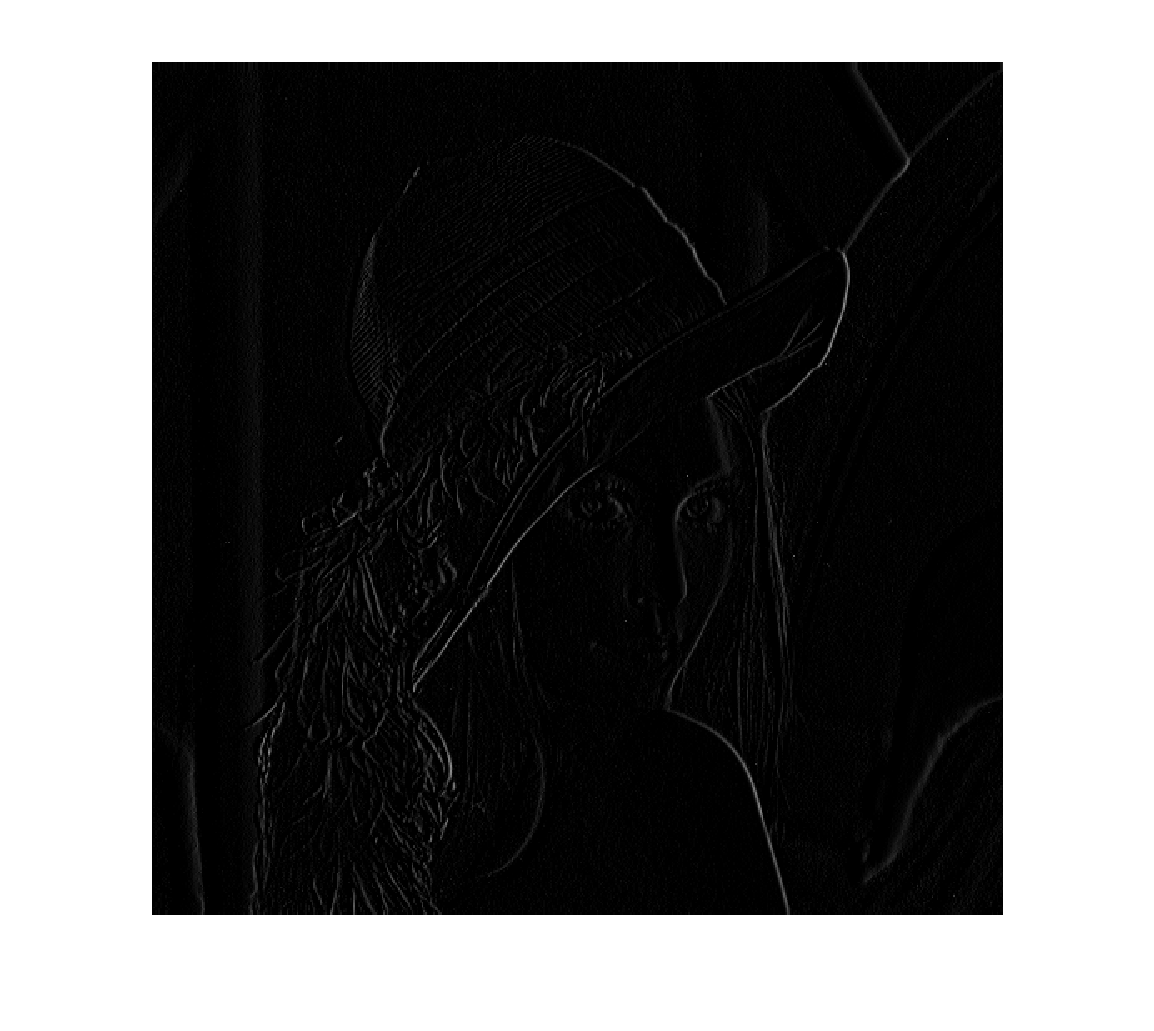
\includegraphics[width=\textwidth]{images/conv2}
                \caption{Matlab's conv2.}
                \label{fig:conv2}
        \end{subfigure}
        \caption{Comparative of the different convolution codes with a horizontal sovel kernel $k = \left[-1, 1 \right]$.}\label{fig:convolution}
\end{figure}

\begin{table}[h]
	\centering
	\begin{tabular}{|c|c|c|c|}
	\hline
     & myconv & myconvFFT & Matlab's conv2 \\ \hline
	Time & 0.658s   & 0.04s     & 0.002s   \\ \hline
	\end{tabular}
	\caption{Performance comparative of the convolution methods.}
	\label{tb:convolutionPerfomance}
\end{table}
 
In Figure~\ref{fig:convolution} we see that the convolution theorem holds, and in Table~\ref{tb:convolutionPerfomance} that performing the operations in the Fourier domain and transforming back is more efficient.

CITE FOURIER TRANSFORM AND CONVOLUTION THEOREM

\section{Features}

Being able to detect features in images that are invariant to rotations, translations, scale and changes in illumination is an useful tool, with many applications such as image matching.
SIFT features CITE LOWE PAPER provide a fairly robust method to detect points in an image with the aforementioned restrictions.
A broad overview of the algorithm is:
\begin{enumerate}
\item \textbf{Extrema detection:} maximum and minimum intensity points are detected in a difference-of-Gaussian pyramid built with the input image.
\item \textbf{Keypoint refinement:} point centrer in interpolated and weak points are rejected.
\item \textbf{Orientation assignment:} orientation and strength of each keypoint are calculated.
\item \textbf{Descriptor calculation:} a 128 feature vector is computed for every element.
\end{enumerate}

\begin{figure}[htbp]
	\centering
	\begin{minipage}[t]{.48\textwidth}
		\centering
		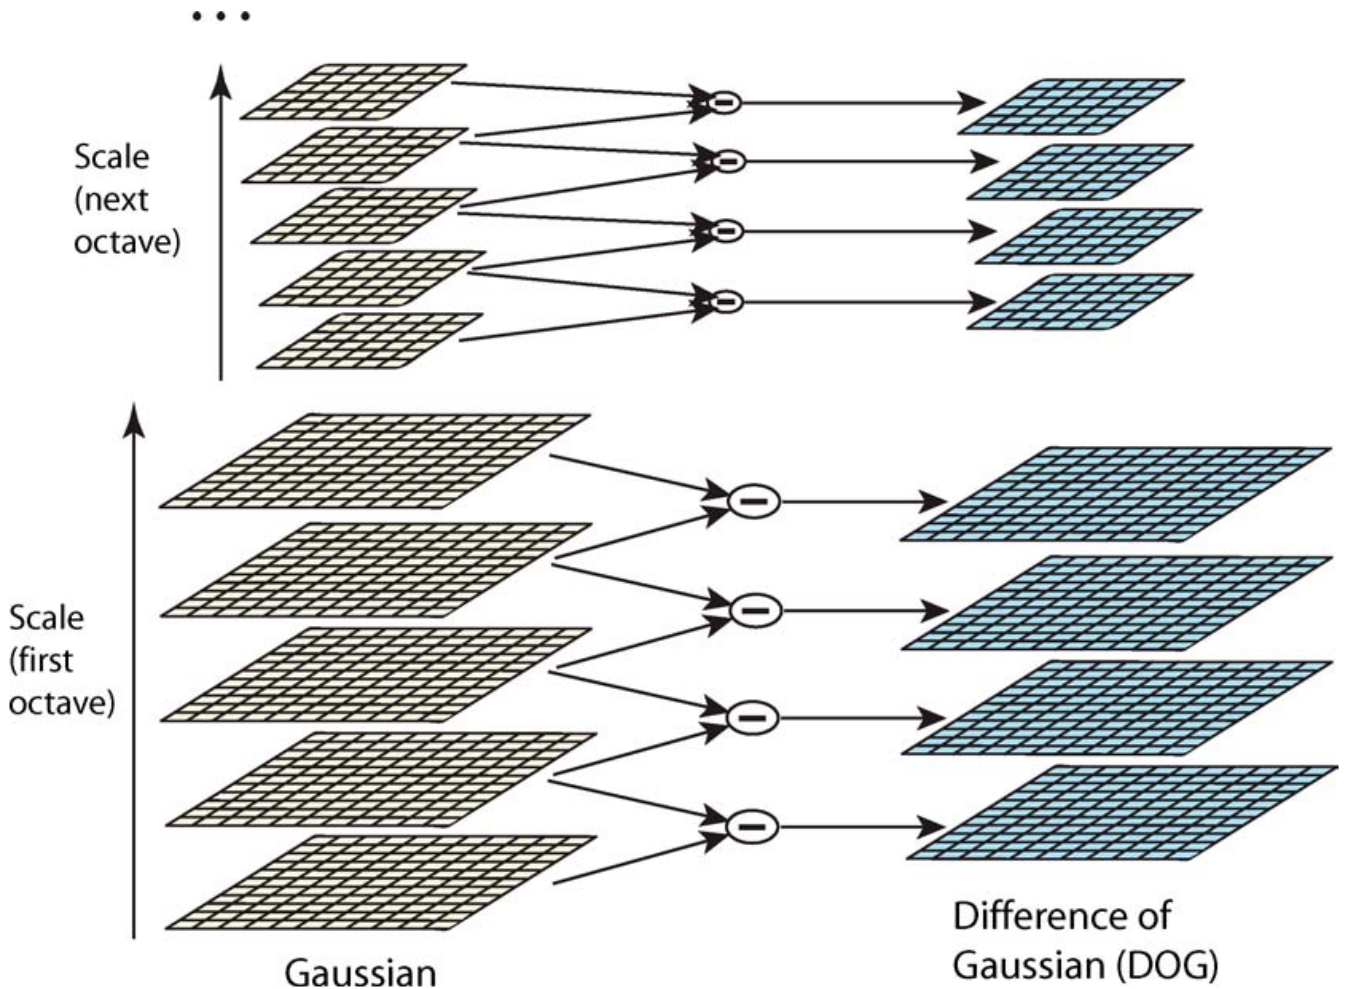
\includegraphics[width=1.05\textwidth]{images/diffOfGauFromPaper}
		\caption{Pyramid of difference-of-Gaussian CITE LOWE.}
		\label{fig:difOfGauPyramid}
	\end{minipage} ~
	\begin{minipage}[t]{.48\textwidth}
		\centering
		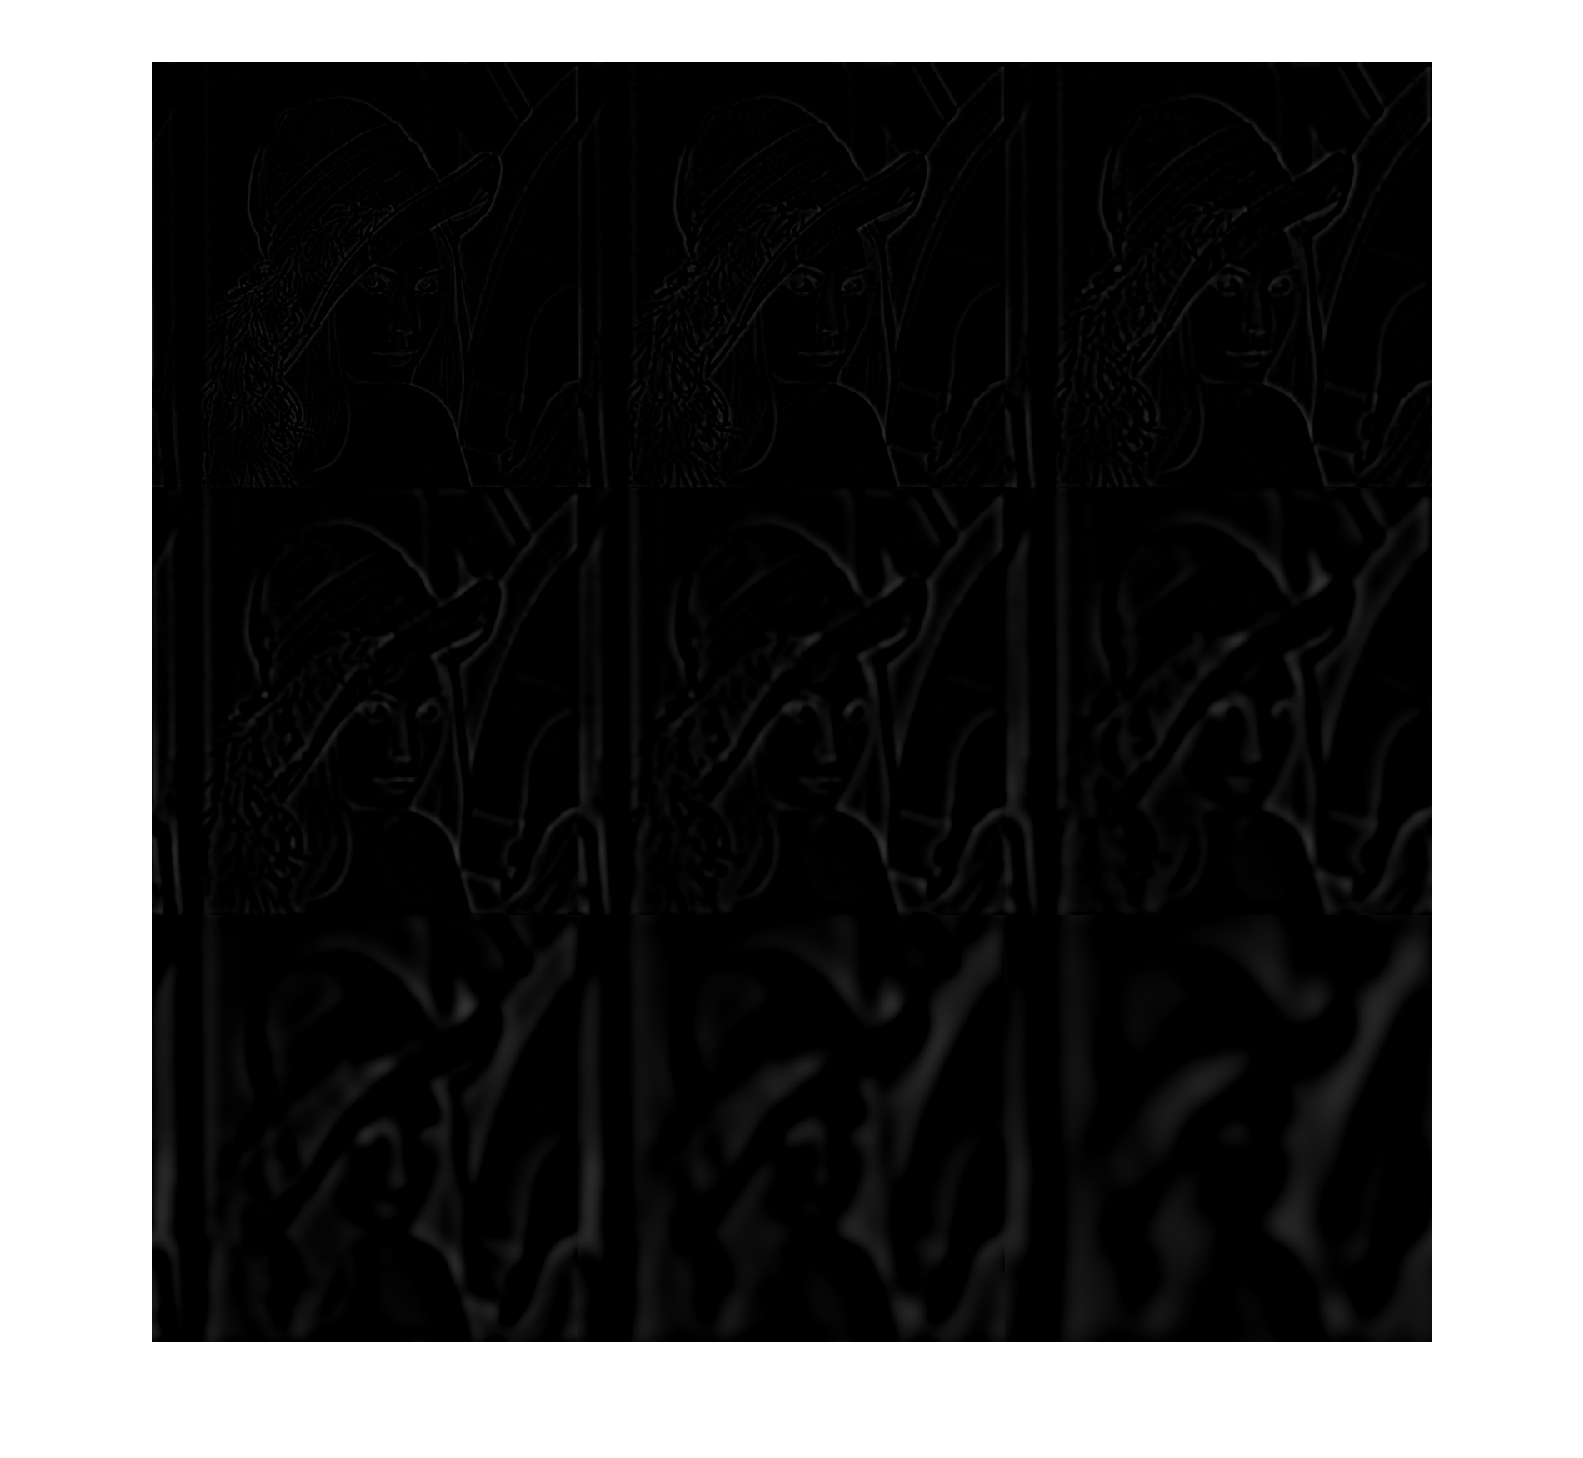
\includegraphics[width=1\textwidth]{images/dogSpace}
		\caption{Example of a scale of a difference-of-Gaussian.}
		\label{fig:difOfGauSample}
	\end{minipage}
\end{figure}

\textbf{Extrema detection} is computed using a difference-of-Gaussian (DOG) structure, as shown in Figure~\ref{fig:difOfGauPyramid}, first a scale of blurred images is constructed.
The input image $I$ is convoluted with a Gaussian kernel $G$:

\begin{equation}
L(x,y,\sigma) = G(x,y,\sigma) * I(x,y),
\end{equation}

where $L$ is the output image, $*$ the convolution operator, $x$ and $y$ the pixel indices, and $G$ and Gaussian kernel defined as:

\begin{equation}
G(x,y,\sigma) = \frac{1}{2 \pi \sigma^2} e^{- \frac{x^2 + y^2}{2 \sigma^2}},
\end{equation}

where $\sigma$ is the standard deviation.
Next, the DOG structure is computed as a difference of several $L$:

\begin{equation}
D(x,y,\sigma) = L(x,y, k\sigma) - L(x,y, \sigma),
\end{equation}

where $D$ is the output image and $k$ is a constant multiplicative factor.
Note that to provide an efficient implementation, the convolution and difference can be computed in the Fourier domain using the convolution theorem explained in Section~\ref{sec:convolution}.
A example on how this DOG structure looks like is shown in Figure~\ref{fig:difOfGauSample}, where the sigma increases from left to right and from top to bottom.
The keypoints selected will be those who are a maximum or a minimum in a $3 \times 3 \times 3$ cube region, so in their scale and the ones above and below.
Selecting locations using this scheme allows to find interested points regardless of their scale, as we progress towards the top of the pyramid,  the local maximum or minima will be produced by bigger objects in $I$.
In our implementation only one scale of the pyramid is calculated.

Keypoint refinement is done with an optimization step which removes weak points and also improves their position.
The new keypoint location $\mathbf{\hat{x}}$ will be:

\begin{equation}
\mathbf{\hat{x}} = - \frac{\partial^2 D^{-1}}{\partial \mathbf{x^2}} \frac{\partial D}{\partial \mathbf{x}},
\end{equation}

where $\mathbf{x}$ is the previous location and $D(\mathbf{x})$ is approximated with a Taylor expansion in the form of:

\begin{equation}
D(\mathbf{x}) = D + \frac{ \partial D^T}{\partial \mathbf{x}} \mathbf{x} + 0.5 \mathbf{x^T} \frac{\partial^2 D}{\partial \mathbf{x^2}}\mathbf{x}.
\end{equation}

Keypoints are rejected if they are weak or in an edge, any extrema is defined as weak if $D(\mathbf{x'}) < 0.03$, where $D(\mathbf{\hat{x}})$ is:

\begin{equation}
D(\mathbf{\hat{x}}) = D + 0.5 \frac{\partial D^T}{\partial \mathbf{x}}\mathbf{\hat{x}}.
\end{equation}

Edge elimination is performed when $R(\mathbf{H}) > f(r)$, where $\mathbf{H}$ is a $2 \times 2$ Hessian matrix, $r = 10$, $R(\mathbf{H})$ is defined as:

\begin{equation}
R(\mathbf{H})= \frac{ (D_{xx} + D_{yy})^2 }{ D_{xx} D_{yy} - (D_{xy})^2} ~ \text{where} ~ D_{\alpha \beta} = \frac{\partial^2 D}{\partial \alpha \partial \beta} ~  \text{for} ~ \alpha, \beta = x, y
\end{equation}

and 

\begin{equation}
f(r) = \frac{(r + 1)^2}{r}.
\end{equation}

\textbf{Orientation assignment} measures the point orientation using local images properties.
The objective is that if a point is rotated in another image, the final descriptor will be the same in both.
A gradient magnitude $m(x,y)$ and orientation angle $\theta(x,y)$ are computed as follows:

\begin{equation}
\begin{aligned}
	m(x,y) &= \sqrt[]{(L(x+1,y,\sigma) - L(x-1,y,\sigma))^2 + (L(x,y+1,\sigma) - L(x,y-1,\sigma))^2}, \\
	\theta(x,y) &= tan^{-1} \left( \left( L(x,y+1,\sigma) - L(x, y-1, \sigma) \right) / \left( L(x+1,y,\sigma) - L(x-1, y, \sigma) \right) \right),
\end{aligned} \label{eq:conv}
\end{equation}

where $L$ is chosen to has the same sigma as the keypoint.

\textbf{Descriptor calculation} uses orientation histograms from sample points near the extrema.
For each keypoint a $16 \times 16$ region around it is chosen and the orientations for each pixel are calculated.
$4 \times 4$ histograms are computed with 8 bins each; this 8-dimensional values are placed in an array forming a 128 element feature vector for each keypoint.
Normalizing the vector to unit length improves invariance to illumination changes.


\begin{figure}[htbp!]
        \centering
        \begin{subfigure}[b]{0.45\textwidth}
                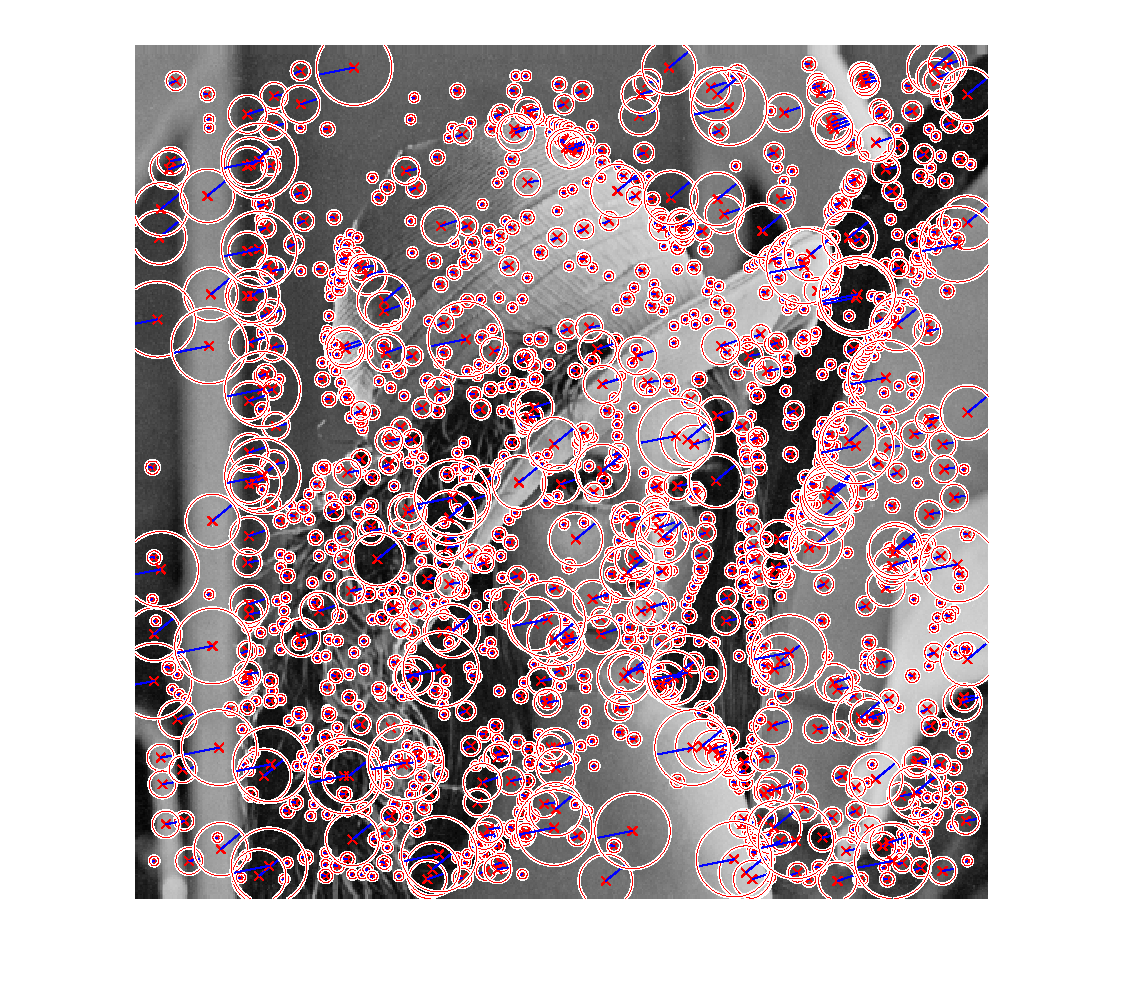
\includegraphics[width=\textwidth]{images/sift2}
                \caption{SIFT without weak and edge keypoint purge.}
                \label{fig:sift1}
        \end{subfigure}
        \begin{subfigure}[b]{0.45\textwidth}
                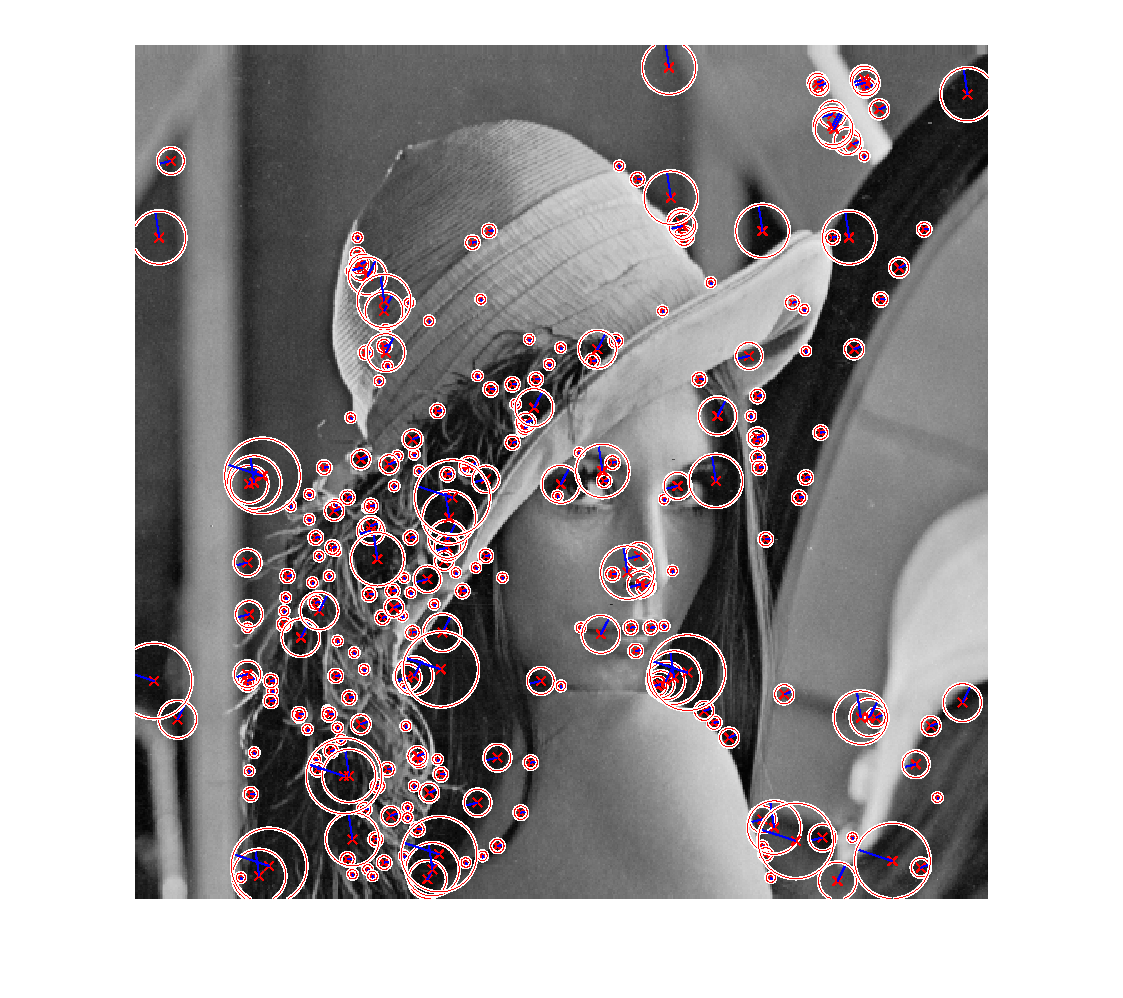
\includegraphics[width=\textwidth]{images/sift1}
                \caption{SIFT with weak and edge keypoint removal.}
                \label{fig:sift2}
        \end{subfigure}
        \begin{subfigure}[b]{0.45\textwidth}
                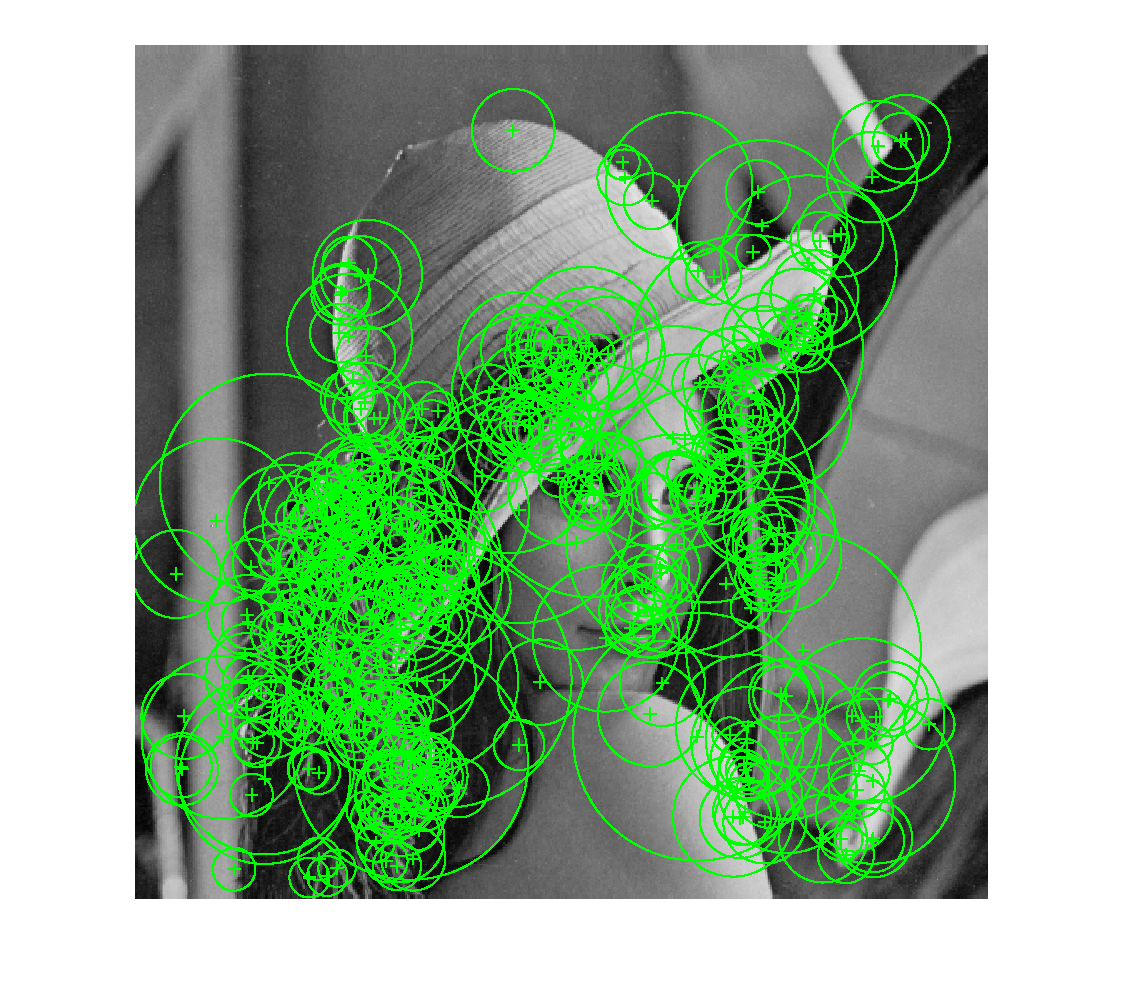
\includegraphics[width=\textwidth]{images/surf1}
                \caption{SURF with default parameters.}
                \label{fig:surf1}
        \end{subfigure}
        \begin{subfigure}[b]{0.45\textwidth}
                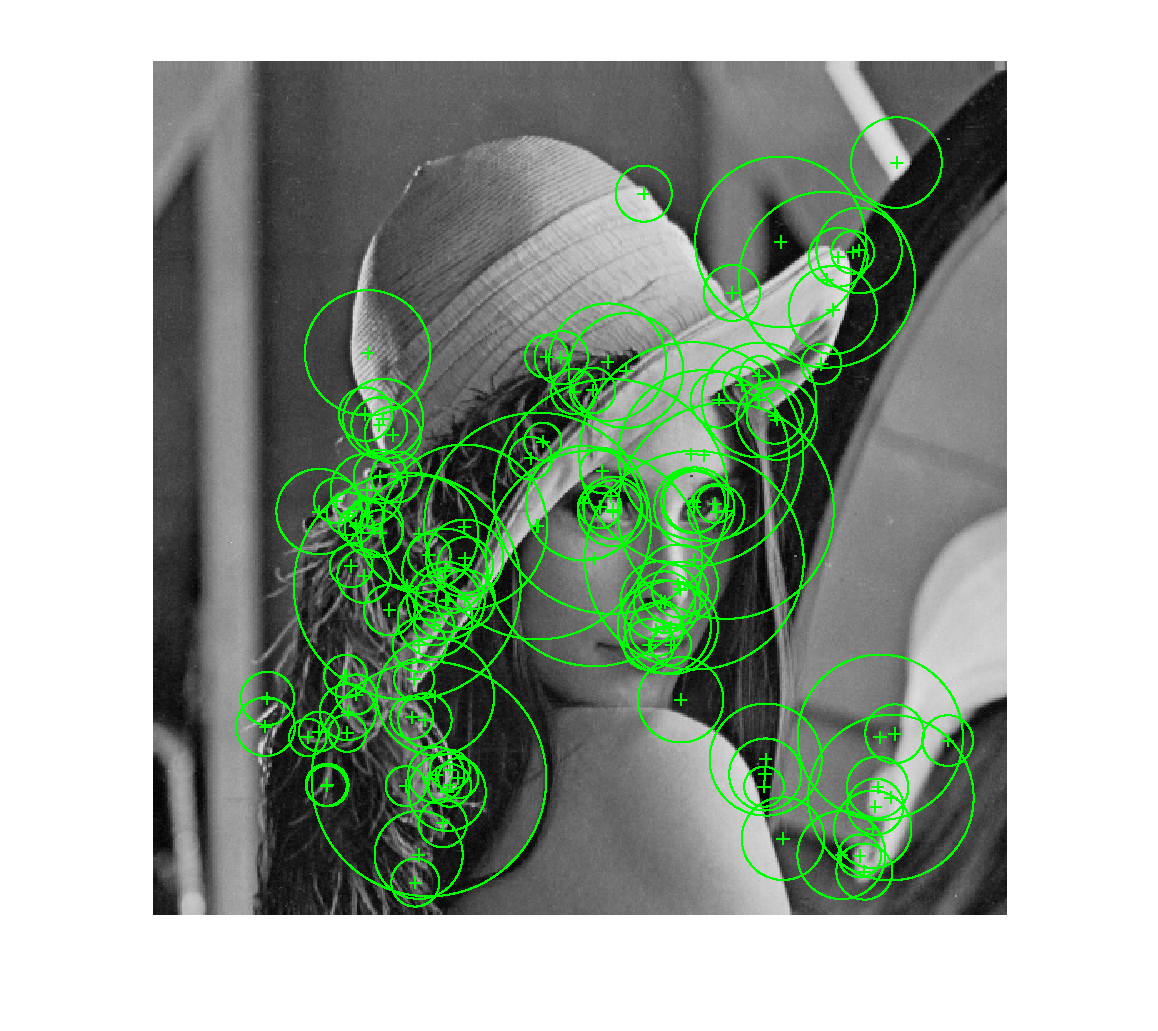
\includegraphics[width=\textwidth]{images/surf2}
                \caption{SURF with the 120 strongest keypoints.}
                \label{fig:surf2}
        \end{subfigure}        
        \caption{Comparative of our SIFT features with Matlab's SURF features.}\label{fig:featuresSample}
\end{figure}

\FloatBarrier % Makes sure the previous figure does not go into the Matching section
\section{Matching}

In the image matching area an image $I_0$ is to be found under a certain affine transformation in another image $I_2$.
The RANSAC (Random Sample Consensus) CITE RANSAC algorithm is a simple and fast approach to perform this task.
Despite being originally designed to estimate the parameters that fit a mathematical model to a dataset which contains outliers, it can also be used to estimate the transformation that matches $I_0$ and $I_1$.

We want to calculate the matrix $H$ that transforms from one image to the other, such that:

\begin{equation}
\begin{bmatrix}
u^* \\ 
v^* \\ 
w^*
\end{bmatrix}
= 
\begin{bmatrix}
 h_{11} & h_{12} & h_{13} \\ 
 h_{21} & h_{22} & h_{23}\\ 
 h_{31} & h_{32} & h_{33}
\end{bmatrix}
\begin{bmatrix}
x \\
y \\
z
\end{bmatrix},
\label{eq:originalH}
\end{equation}

where $u^*$, $v^*$ and $w^*$ are the scaled pixel coordinates in $I_1$ and $x$, $y$ and $z$ the scaled pixel coordinates in $I_0$.
Collecting $H$ in rows, $H_i = \begin{bmatrix} h_{i1} & h_{i2} & h_{i3} \end{bmatrix}$ for $i = \lbrace 1,2,3 \rbrace$ and $\mathbf{x} = \begin{bmatrix} x & y & z \end{bmatrix}$ we can rewrite Equation~\ref{eq:originalH} into:

\begin{equation}
\begin{aligned}
	u^* = H_1 \mathbf{x}, \: v^* &= H_2 \mathbf{x}, \: w^* = H_3 \mathbf{x}, \\ 
	\text{enforcing} \: w^* &= 1, \\
	u = \frac{H_1 \mathbf{x}}{ H_3 \mathbf{x}}, \: v &= \frac{H_2 \mathbf{x}}{ H_3 \mathbf{x}}, \: \text{hence} \\
	uH_3\mathbf{x} - H_1\mathbf{x} &= 0, \\
	vH_3\mathbf{x} - H_2\mathbf{x} &= 0.
\end{aligned}
\end{equation}

As shown in the previous equations, each match provides two equations to solve $H$.
Since, we enforce the scale to be a homogeneous coordinate, $h_{33} = 1$ is no longer an unknown.
For eight unknowns, eight equations are needed, so four points in each image are to be matched.
In matrix notation, we will stack all the equations in a matrix $A$, such that $A\mathbf{h}=0$, where $\mathbf{h}$ is $H$ reshaped into a column vector.
Singular value decomposition of $A$ can be computed to solve the system, $A = UZV^T$, where $U$ and $V$ are unitary, $Z$ is rectangular diagonal and $\mathbf{h} = V_{i9}$ for $i = \lbrace 1,2, \ldots, 9 \rbrace$.

\section{Reconstruction}

\end{document}

\section{Results}
